%Simulation Results and Discussion


\subsection{Length of shortest tour}

In a first attempt the dependency of the shortest tour length on different parameters is analysed. Thereby the number of completed rounds each agent finishes is varied. Moreover the relative weighting of deposited pheromone and closeness is analysed by changing the parameter \beta and the value of the update rate \alpha is optimized. \\
The shortest tour length is calculated for a 30 and 51 cities problem and averaged over 10 trials. In Figure \ref{fig:roundspeil} and \ref{fig:roundspoli} its dependency on the number of completed tours is shown. As expected the average length decreases asymptotically towards the value of the optimal path. For both city environments the program achieved to reach the averaged shortest path known from literature \cite{paper} and \cite{oli}. For thirty cities and 400 rounds, $<$shortest path$>$ is in fact equal the best result found, whereas for 51 cities a lot more rounds would have been needed to achieve this. Anyhow, the best result obtained in a single run is $<\text{shortest path}>=429.48 \pm 1.86$.\\In Figure \ref{fig:roundspeil} three models have been implemented and tested. The first (white circle dots) correspond exactly to the one described in \cite{paper} where all agents are moving at the same time step. The red squares represent the result obtained by a slightly modified model. The same mathematics has been used but the agents are exploring a new trail one by one. As can be seen, this change has little effect on the value of the shortest tour length and its error.\\ Adapting the pheromone update equations (\ref{eq:localtauupdate}) and (\ref{eq:globalupdate}) on page \pageref{sec:model} by adding a constant of 0.1, results in a steeper fall of the average shortest path. At 2000 rounds the final value does not yet reach the averaged shortest path length from \cite{paper}. One concludes that the added constant was chosen too high such that the global and local update only had a neglecting influence on $\tau(r,s)$.\\

The trajectory vector of the shortest tour, i.e. the sequence of city numbers which yields the optimal tour .

This value is then compared to the known solution from \cite{web:data} and \cite{web:oli}. This is also done with 

\begin{figure}[h!]
\begin{center}
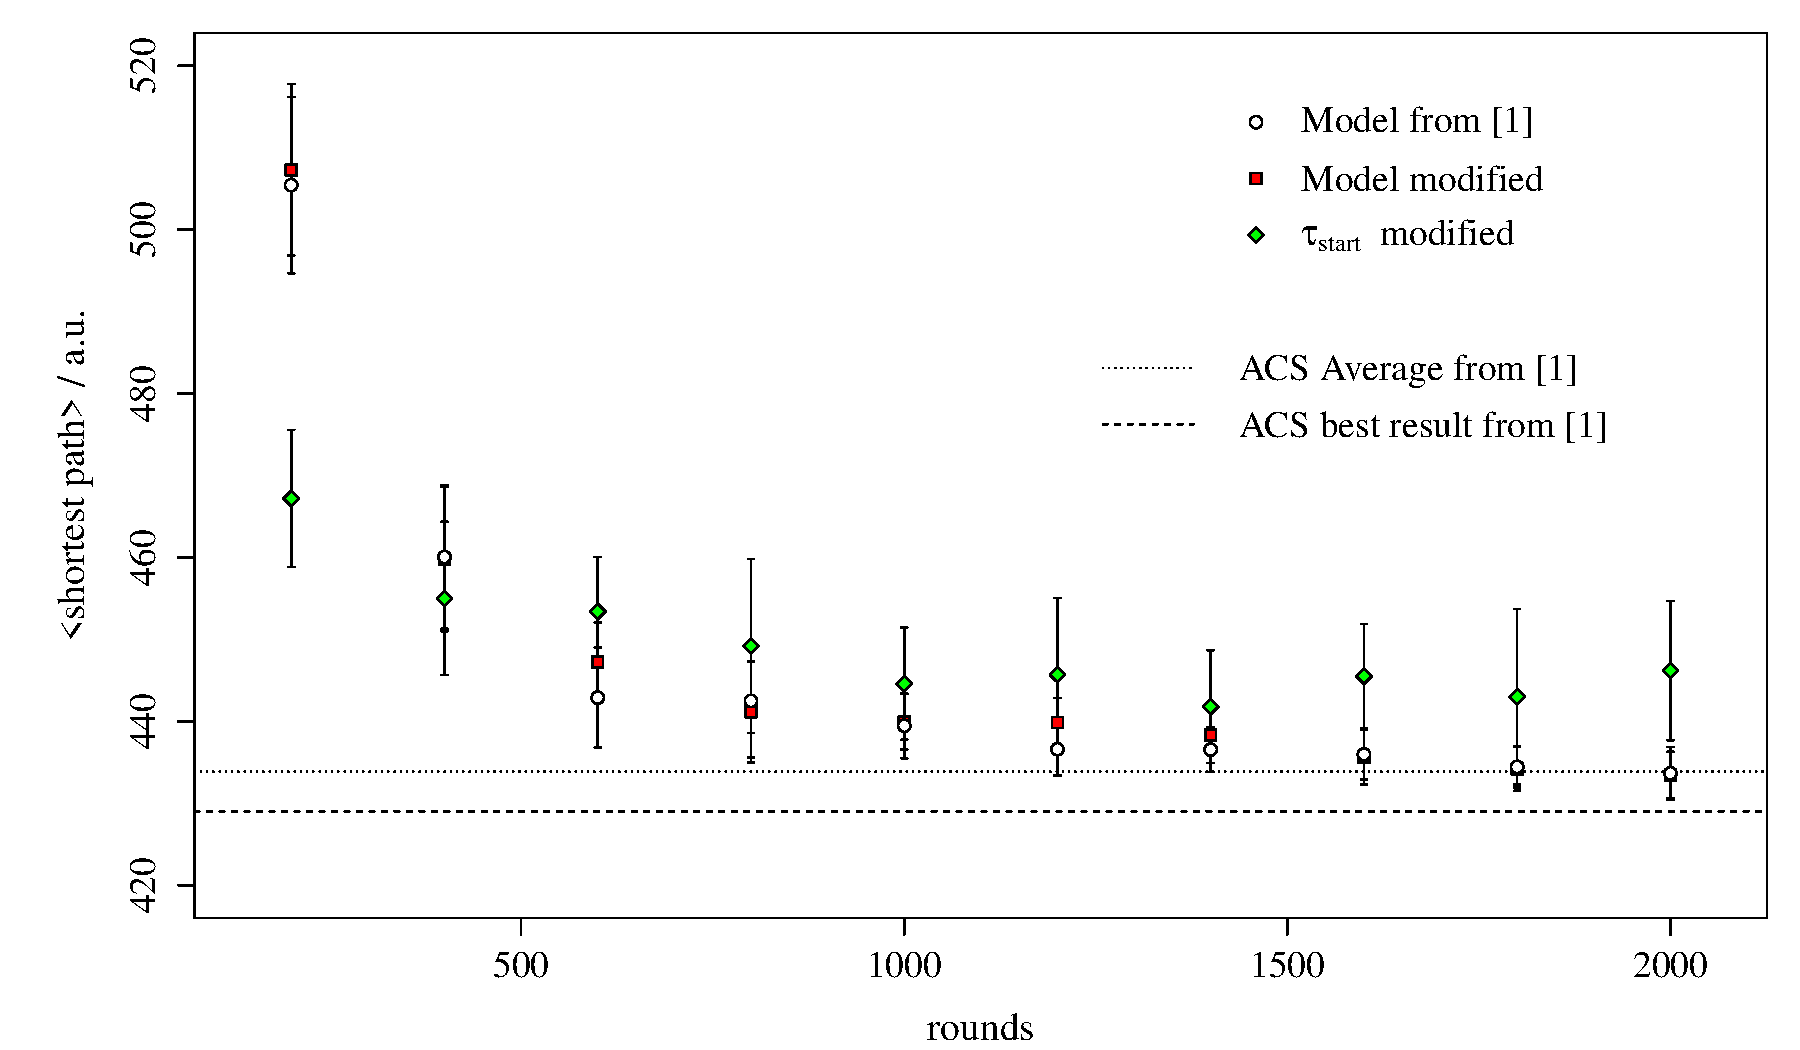
\includegraphics[width=11cm, height= 6 cm]{rounds_vs_shortestpath_eil}
\caption{Shortest tour length averaged over 10 runs for different numbers of rounds. The value approximates the optimal solution for \approx 1200 rounds.}
\label{fig:roundspeil}
\end{center}
\end{figure}


\begin{figure}[h!]
\begin{center}
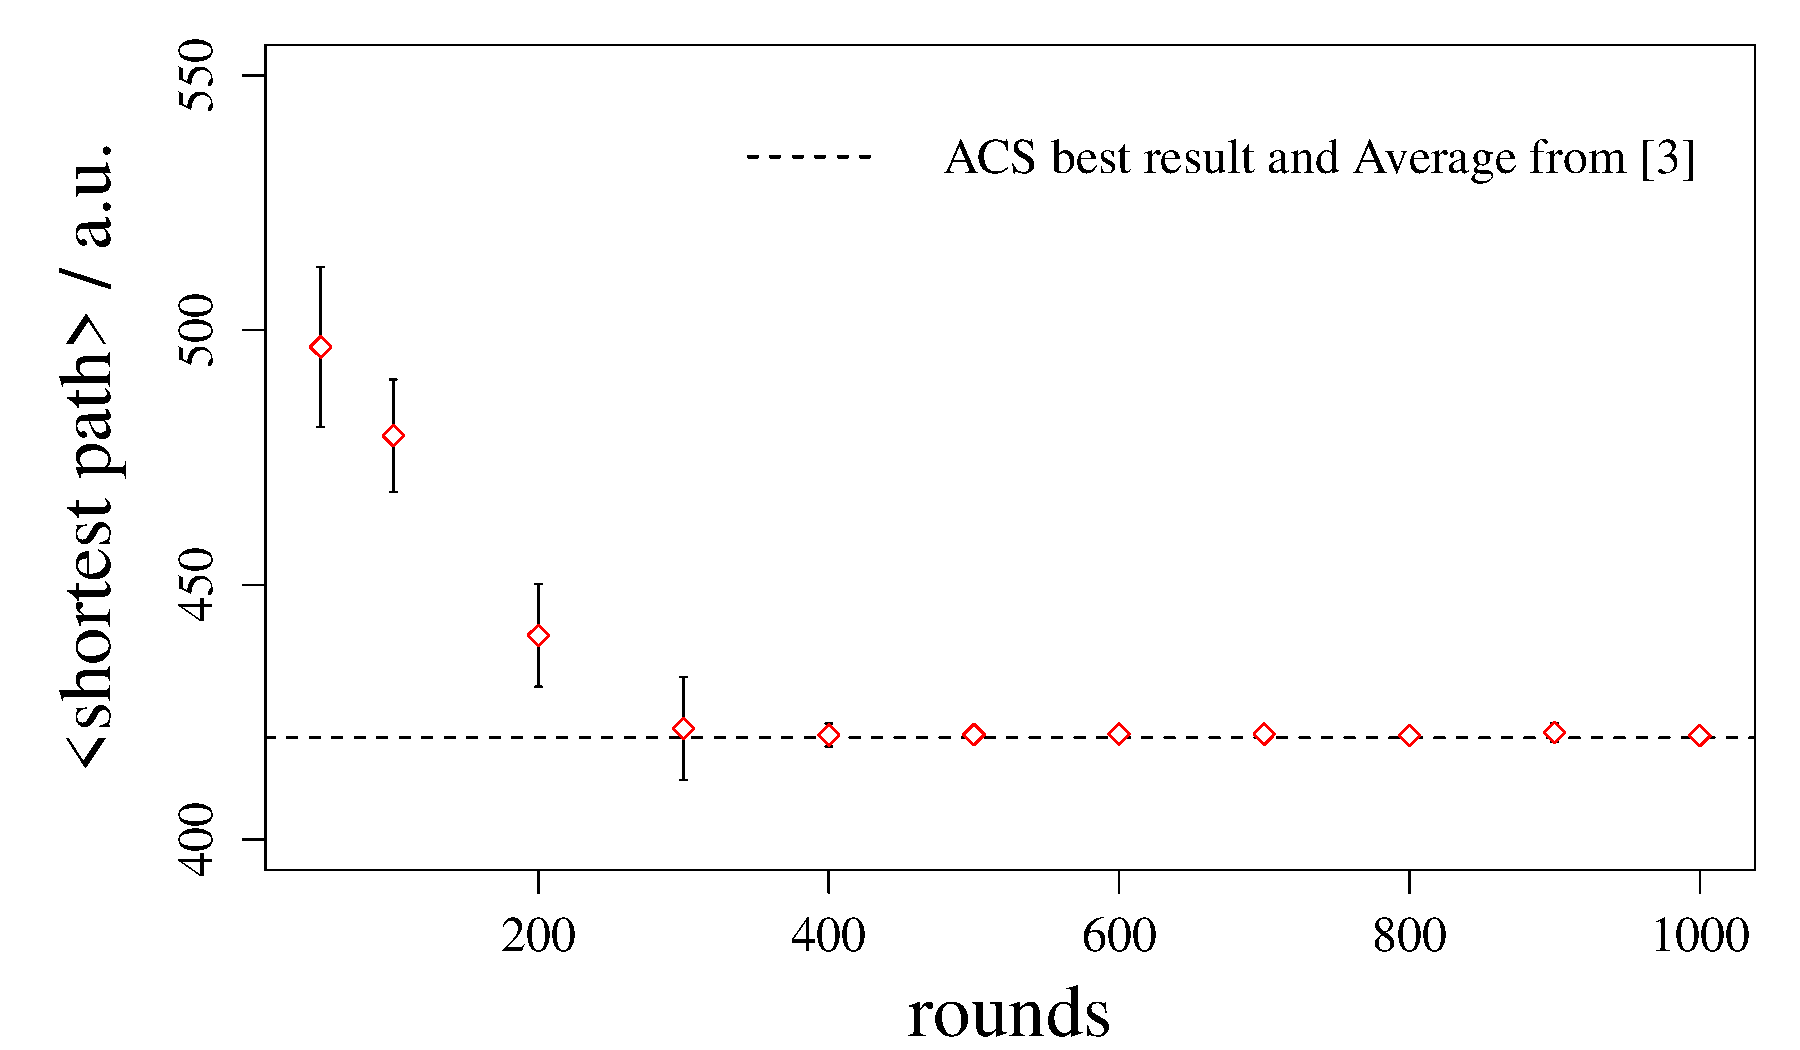
\includegraphics[width=11cm, height= 6 cm]{rounds_vs_shortestpath_oli}
\caption{Shortest tour length averaged over 10 runs for different numbers of rounds. The value approximates the optimal solution for \approx 400 rounds.}
\label{fig:roundspoli}
\end{center}
\end{figure}


Figure \ref{fig:alphasp} illustrates that the averaged shortest path length is optimized for \alpha between 0.1 and 0.3. This is the region where the length of the tour and also the error of the shortest path is minimized. The reason why the shortest path is highest close zero and one, can be understood considering the pheromone update formulas (\ref{eq:localtauupdate}) and (\ref{eq:globalupdate}) on page \pageref{sec:model}. For $\alpha=0$ the local and global pheromone concentration stays constant, no update is made. Hence the cities are only favored by closeness and not by the pheromone concentration anymore. On the other hand, if \alpha is close to one the amount of pheromone after the local update has changed a lot. Randomly chosen trails which deviate from the shortest path will be weighted too much. Therefore the optimal update rate \alpha is expected to be closer to zero. 
\begin{figure}[h!]
\begin{center}
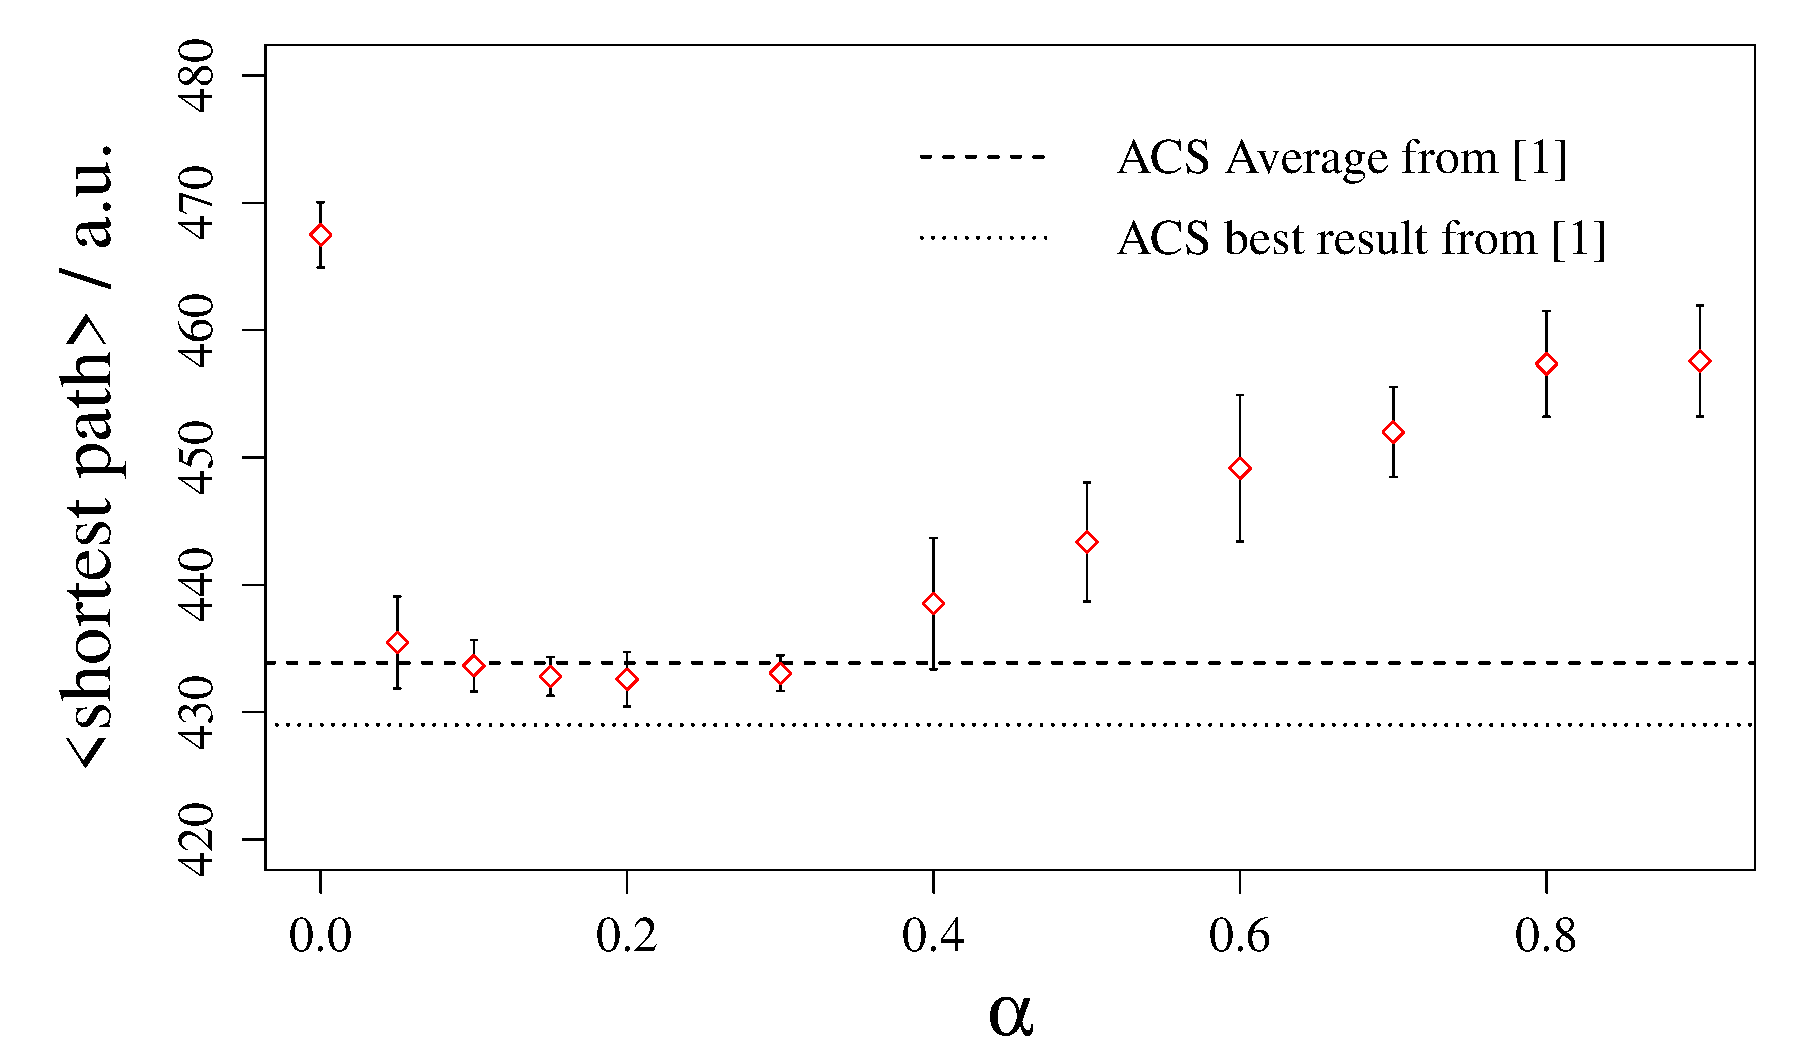
\includegraphics[width=11cm, height= 6 cm]{alpha_vs_shortestpath}
\caption{The update rate parameter \alpha changes the averaged shortest tour length. The simulation is done for a fifty city problem using ten agents which all completed 2000 rounds. Other parameters are set to $beta=2$, $q_0=0.9$ and $tau_{\ref{start}}=0.1$. The values are averaged over ten runs. By setting $\alpha=0.1$ the length of the averaged shortest path is comparable to the value found in literature \cite{paper} and the change in pheromone update is held low.}
\label{fig:alphasp}
\end{center}
\end{figure}

For the parameter \beta a similar analysis has been done for a thirty city environment and ten agents. The motivation for setting $\beta=2$ in \cite{paper} is barely understood from figure \ref{fig:betasp}. The decrease of the error for higher values of \beta is explained by the fact that the criteria of closeness between the cities is weighted stronger than the pheromone concentration (see equation (\ref{eq:prob}) and (\ref{eq:qsmallerq0})). Thus, the exploration of new paths is suppressed and the deviation from the averaged path length is small. In the region of $beta\approx2$ the bigger error bars indicate that the relative importance of pheromone and closeness is chosen such that the ants are forced to try new trails. The probability of getting stuck in a local minimum is reduced.
\begin{figure}[h!]
\begin{center}
\includegraphics[width=11cm, height= 6 cm]{abeta_vs_shortestpath}
\caption{Variation of the parameter \beta for the oliver30 using ten ants going 400 rounds averaged over 20 runs. The parameters are chosen as $\alpha=0.1$,$q_0=0.9$ and $tau_{\ref{start}}=0.1$.}
\label{fig:betasp}
\end{center}
\end{figure}



\subsection{Model adaptions}

